\chapter{Contributions to Spot}

This chapter present the different things I have done on Spot during the internship. Might it be
some algorithms implemented, scripts, display arrangements, benchmarks, results analyzes, etc.

\noindent All the achieved work is presented in a chronological way, to bring out the difficulties
encountered, the unexpected results that had influence on the advancement of the work.

\section{fastSAT}
As a quick reminder, here are the required characteristics for the SAT solver:
\begin{itemize}
 \item licence compatibility with Spot's one (GNU GPL v3),
 \item simplicity of integration for future updates,
 \item effectiveness.
\end{itemize}

\noindent The project \textbf{fastSAT}\cite{5} was born to help choose the SAT solver to distribute with
Spot. Until now, SAT-based minimization was performed through an external SAT solver. The default one
was Glucose \cite{12} (3.0 version). Therefore, it seems logical to consider Glucose as a possible
candidate. \textbf{fastSAT}\cite{5} compared Glucose 4.0 \cite{12} to CryptoMiniSat 5.0.1\cite{20} and
PicoSAT 965 \cite{21}. Note that some SAT solvers provide two versions, one parallal and one simple
essentially because of the SAT competitions. In short, were compared:
\begin{itemize}
 \item Glucose syrup (parallal) 4.0
 \item Glucose simple 4.0
 \item CryptoMiniSat parallal 5.0.1
 \item CryptoMiniSat simple 5.0.1
 \item PicoSAT 965
\end{itemize}

The next three figures (\ref{fig:satchoose_1}, \ref{fig:satchoose_2} and \ref{fig:satchoose_3}) show some
comparaisons for three formulas. About twenty formulas have been tested in two modes: by forcing the number
of state and by doing the complete cycles of minimization. It has been executed on a computer with an
\textbf{Intel(R) Core(TM) i7-4710HQ CPU @ 2.50GHz} processor and  a \textbf{8 GiB} system memory.
The measuring tool used is the open Google Benchmark tool \cite{22}.

\begin{figure}[H]
 \centering
 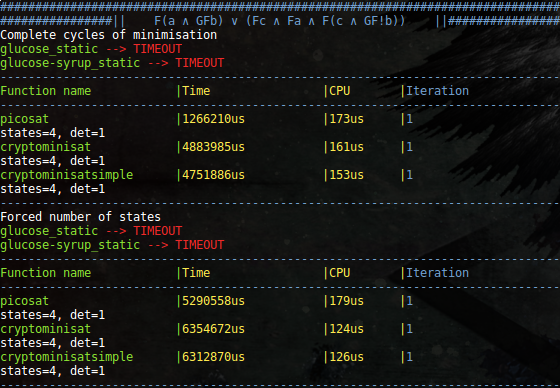
\includegraphics[scale=0.7]{img/satchoose_1.png}
 \caption{Benchmark for formula $F(a \land GFb) \lor (Fc \land Fa \land F(c \land GF(!b)))$}
 \label{fig:satchoose_1}
\end{figure}

\begin{figure}[H]
 \centering
 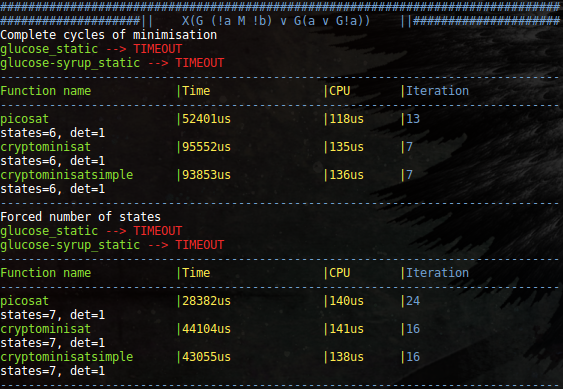
\includegraphics[scale=0.7]{img/satchoose_2.png}
 \caption{Benchmark for formula $X(G (!a M !b) \lor G(a \lor G(!a)))$}
 \label{fig:satchoose_2}
\end{figure}

\begin{figure}[H]
 \centering
 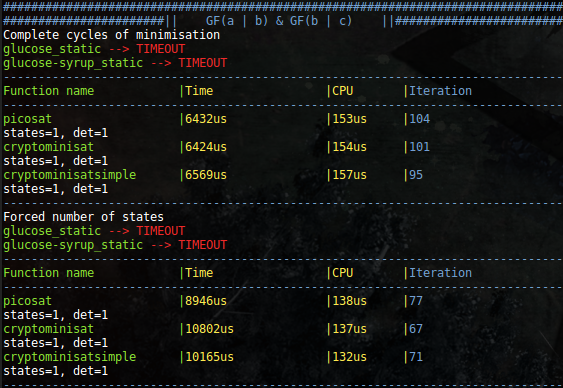
\includegraphics[scale=0.7]{img/satchoose_3.png}
 \caption{Benchmark for formula $GF(a \lor b) \land GF(b \lor c)$}
 \label{fig:satchoose_3}
\end{figure}

\noindent In conclusion, among the different SAT solvers, \textbf{PicoSAT} was choosen for its strong
performances. It consists of two source code files: \textbf{picosat.h} and \textbf{picosat.c} and was
easily integrated and harmonised with Spot.

\textbf{fastSAT}\cite{5} project is fully availlable and anyone can reproduce the benchmarks. Feel free to
have a look.

\section{New Satsolver class}
There was already a satsolver class that is instantiated at the beginning of the SAT-based minimization
procedures, formerly used to initialize a temporary \textbf{cnf file} (DIMACS \cite{18}), return
it and call the external SAT solver. The file writing was directly made by those procedures.

\noindent The objective is to completely abstract the file writing. SAT-based minimization procedures will
just have to instantiate a satsolver object at the beginning and make calls to its functions. Thoses
functions will call the SAT solving library functions. But this class must continue to support any external
SAT solver by handling temporary \textbf{cnf files}.\\

\begin{figure}[h]
  \centering
  \begin{tikzpicture}
    \begin{umlpackage}{Pseudo UML}
     \umlclass[name=satsolver, template=T]{spot::satsolver}
     {
       psat\_ : PicoSAT*\\
       cnf\_stream\_ : std::ostream*\\
       nb\_clauses\_ : int\\
       nb\_vars\_ : int\\
       ...
       }{
       add(std::initializer\_list\textless int\textgreater values : void\\
       add(int v) : void\\
       comment(T first, Args... args)\\
       get\_nb\_clauses() : int\\
       get\_nb\_vars() : int\\
       get\_solution() : std::pair\textless int, std::vector\textless bool\textgreater\textgreater\\
       ...
     }
    \end{umlpackage}
  \end{tikzpicture}
  \caption{Satsolver class UML representation}
  \label{fig:sat_uml}
\end{figure}

\noindent The figure \ref{fig:sat_uml} shows an approximate UML representation of the new satsolver class.
It can either initialize PicoSAT or a cnf\_stream\_. The idea is to let its functions (add, comment, etc.)
to decide if they call PicoSAT functions or write in the cnf\_stream\_. That way, SAT-based minimization
procedures are not aware of what's going on behind and can repeat over and over again the same algorithms.\\

\noindent Of course the clause counting mechanism is provided by the new satsolver class. At the end,
SAT-based procedures will just have to call the \textit{get\_solution()} method.\\

Once this was done, SAT-based procedures had already gained some speed which is entirely understandable as
disk operations are slow. For instance, with this command
line:
\begin{lstlisting}[language=bash,caption={bash command-line to test a formula minimization using ltl2tgba}]
  time ltl2tgba -D -x sat-minimize 'G(a -> Fb) & G(c -> Fd)'
                        --stats='states=%s, det=%d'
\end{lstlisting}
This result is obtained on a Macbook pro with \textbf{2,9GHz intel core i5} and
\textbf{8 Go 1867 Mhz DDR3}:\\\\
\begin{tabular}{|c|c|}
 \hline
 &\\
 PicoSAT as & Time result\\
 &\\
 \hline
 &\\
 linked SAT solving library&0.29s user 0.08s system 98\% cpu 0.371 total\\
 external SAT solver (with disk operations)&0.82s user 0.09s system 98\% cpu 0.925 total\\
 &\\
 \hline
\end{tabular}

\section{First incremental approach}
\label{approach1}
Just as a reminder, until now, SAT-based minimization procedures whether it is with binary search
(algorithm \ref{dicho}) or the naive way (algorithm \ref{naive}), starts the SAT encoding from scratch
at each step of the cycle of minimization; that is unfortunate. This is why an incremental approach
has been considered.\\

\noindent  The algorithm \ref{incr1} has been implemented. Starting with an $\omega$-automaton of size
$n$, if the first iteration (which encodes the research of an $\omega$-automaton of size $n-1$) constructs
an automaton of $k$ ($k \leq n-1$) states \textit{accessible}, then some clauses are added to forbid all the
entrant transitions of the $n-k-1$ last state. If such automaton is found, the entrant transitions of the
$n-k-2$ last state are also forbidden, etc. The last SAT problem solved correspond to the minimal
automaton.\\

\noindent An interesting thing, as a sideline, is that at the beginning, instead of forbidding the entrant
transitions of a state, the outgoing transitions were forbidden. This did not work, because those
clauses were in contradiction with the first rule of the encoding (which stated that the automaton must be
\textit{complete}), causing an absurdity. All the rules of the encoding are described in the papers
\cite{14} and \cite{15}.\\

\noindent After this method has been implemented (algorithm \ref{incr1}), a benchmark has been realized to
compare it to the old default method (algorithm \ref{naive}). For dispay reasons, only a few interesting
lines of the results are displayed in the figure \ref{fig:glu_vs_incr1_short}. Feel free to have a look
in the \ref{glu_vs_incr1_complete} section of the appendix to see all the results. For each version and
each formula, two minimizations are attempted, büchi \textit{acceptance set} and
\textit{generalized büchi acceptance set}. The best performances for each formula are colorized
respectively in green and yellow.

\begin{figure}[H]
 \centering
 \fontsize{9}{11}\selectfont{
 \setlength\LTleft{0pt}% default: \parindent
 \setlength\LTright{0pt}% default: \fill
 \begin{longtable}{@{\extracolsep{\fill}}|*{5}{c|}}
  \hline
  \multirow{3}{*}{Formulas}&\multicolumn{4}{c|}{Time (seconds)}\\
  &\multicolumn{2}{c|}{Glucose (As before)}&\multicolumn{2}{c|}{Incr Naive}\\
  &minDBA&minDTGBA&minDBA&minDTGBA\\
  \hline
  $F(a \land  GFb) \lor  (Fc \land  Fa \land  F(c \land  GF\bar b))$&0.02&\cellcolor{Yelw} 57.65&\cellcolor{Green} 0.01&236.36\\
  $XXG(Fa U Xb)$&25.15&\cellcolor{Yelw} 762.74&\cellcolor{Green} 20.21&(killed)\\
  $(a R (b R Fc)) W XGb$&(killed)&\cellcolor{Yelw} 254.19&(killed)&672.80\\
  $X(\bar a \land  Fa) R (a M Fb)$&2.19&\cellcolor{Yelw} 46.12&\cellcolor{Green} 1.7&132.02\\
  $(a R Fb) U X\bar c$&(killed , $\le$ 11)&\cellcolor{Yelw} 389.87&(killed , $\le$ 11)&616.70\\
  \hline
 \end{longtable}}
 \caption{Parts of \ref{glu_vs_incr1_complete} benchmark results showing some cases where the Old SAT-based
          minimization is still better}
 \label{fig:glu_vs_incr1_short}
\end{figure}

In all the lines of the figure \ref{fig:glu_vs_incr1_short}, \textbf{glucose} is still better than our first
incremental approach. There is even a case where \textbf{naive incr} never ends the minimization and
is killed.

In order to better compare both version, this generated figure counts the number of times a version is
better than the other with a tolerance of more or less five percents (5\%). That means: roughly equal times
are skipped.
\begin{figure}[H]
 \centering
 \begin{tabular}{|c|c|c|c|}
\hline
\multicolumn{4}{|c|}{DBA}\\
\hline
&glu&incr1&total\\
\hline
glu&{-}&9&9\\
\hline
incr1&102&{-}&102\\
\hline
\multicolumn{4}{c}{}\\
\hline
\multicolumn{4}{|c|}{DTGBA}\\
\hline
&glu&incr1&total\\
\hline
glu&{-}&8&8\\
\hline
incr1&93&{-}&93\\
\hline
\end{tabular}
 \caption{Summary of \ref{glu_vs_incr1_complete} benchmark}
 \label{fig:glu_vs_incr1_resume}
\end{figure}

The next two figures (\ref{fig:glu_vs_incr1_dba} and \ref{fig:glu_vs_incr1_dtgba}) shows two graphs generated
with ggplot2 \cite{23} (a graphing package implemented in top of the \textbf{R} statistical package). Any
point between the two lines passing through the origin is in the tolerance area (more or less 5\%). All the
bothering points (cases where glucose win) are located in the area over both lines. Obvisouly, the
first incremental approach wins when points are located under both lines.

\begin{figure}[H]
 \centering
 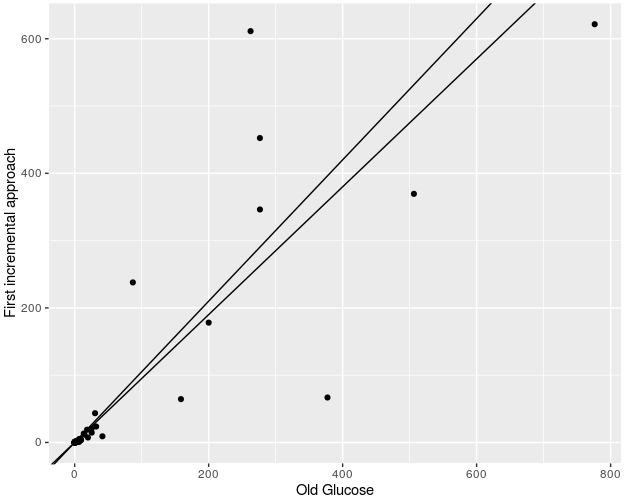
\includegraphics[scale=0.6]{img/glu_vs_incr1_dba.png}
 \caption{Graph comparing both minDBA time of minimization}
 \label{fig:glu_vs_incr1_dba}
\end{figure}

\begin{figure}[H]
 \centering
 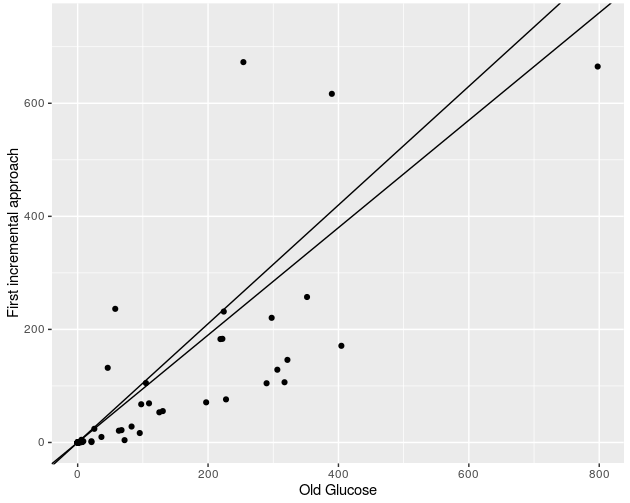
\includegraphics[scale=0.6]{img/glu_vs_incr1_dtgba.png}
 \caption{Graph comparing both minDTGBA time of minimization}
 \label{fig:glu_vs_incr1_dtgba}
\end{figure}

\noindent In light of the above, this incremental approach does not seem to be the most appropriate method.
This is really surprising. Why all that the SAT solver learned while solving the first traditional encoding
did not help him to solve quickly the next similar problems?\\

An hypothesis raised is that may be the fact that the size of the problem is never decreased affect it? By
restarting the encoding from scratch at each step, the Old SAT-based minimization also restarts with a
smaller automaton. The smaller the input automaton is, the smaller the SAT problem produced is (with a
decreasing number of litterals and clauses).\\

As SAT competitions also compares SAT solvers in incremental mode, they have defined a file format,
called XCNF. As our incremental scenarios seem to offer challenges to SAT solver, we decided to provide
a way to generate XCNF file corresponding to complete cycles of this first incremental minimization. We thus
hope that SAT solvers contributors will think about how to improve their solver to be efficient in
these incremental SAT solving scenarios.

\section{A not total incremental approach}
\label{approach2}
With a view to verify the last hypothesis, a similar approach has been proposed.
The idea is to provide the opportunity to choose how many times SAT-based
minimization should work incrementally before restarting the encoding from scratch. Here times can be seen
in two ways. It can be either the number of states to reduce or just a number of attemps before
restarting the encoding. The second way has been chosen because gaining many states when only one is
expected is unpredictable.\\

Here is how the algorithm looks like ($s$ means sat\_incr\_steps and stands for the number of attempts).

\begin{algorithm}[H]
 \caption{This incremental approach attemps a traditional encoding and then tries to exclude
          $s$ states incrementally before restarting the encoding from scratch.}
 \label{incr2}
 \begin{algorithmic}[1]
  \Procedure{\textsc{ReduceStatesDTGBA}$(R,m=R$.nb\_acc\_sets()$, s)$}{}
   \BState \emph{repeat}:
   \State{$n \gets R.nb\_states() $}
   \State{$C \gets \textsc{Synthetize}DTGBA(R,n-1,m) $}
   \If{$C$ \textbf{does not exists}} \Return $R$\EndIf
   \For{$i = 0$; $i < s;$ ++$i$}
    \State{add clauses to exclude one more state}
    \State{$C \gets$ Try to solve the new problem and build the new automaton}
    \If{$C$ \textbf{does not exists}} \Return $R$\EndIf
    \State{$R \gets C$}
   \EndFor
  \EndProcedure
 \end{algorithmic}
\end{algorithm}

Again, once this was implemented, a new benchmark was made. Different values for $s$ has been tested:
$1, 2, 4$ and $8$, $2$ was the best value between them. Again, for some display reasons, only this version
is displayed in comparaison to the Old SAT-based minimization in the figure \ref{fig:glu_vs_incr2_short}
and in the appendix \ref{glu_vs_incr2_complete}.

\begin{figure}[H]
 \centering
 \fontsize{9}{11}\selectfont{
 \setlength\LTleft{0pt}% default: \parindent
 \setlength\LTright{0pt}% default: \fill
 \begin{longtable}{@{\extracolsep{\fill}}|*{5}{c|}}
  \hline
  \multirow{3}{*}{Formulas}&\multicolumn{4}{c|}{Time (seconds)}\\
  &\multicolumn{2}{c|}{Glucose (As before)}&\multicolumn{2}{c|}{Incr Naive}\\
  &minDBA&minDTGBA&minDBA&minDTGBA\\
  \hline
  $F(a \land  GFb) \lor  (Fc \land  Fa \land  F(c \land  GF\bar b))$&0.02&\cellcolor{Yelw} 57.65&\cellcolor{Green} 0.01&237.43\\
  $XXG(Fa U Xb)$&25.15&\cellcolor{Yelw} 762.74&\cellcolor{Green} 12.48&(killed)\\
  $(a R (b R Fc)) W XGb$&(killed)&\cellcolor{Yelw} 254.19&(killed)&778.38\\
  $G(XX F a U (a \lor b \lor Fc))$&\cellcolor{Green}262.56&(killed)&501.21&(killed)\\
  $X(\bar a \land  Fa) R (a M Fb)$&2.19&\cellcolor{Yelw}46.12&\cellcolor{Green}1.71&129.43\\
  $(a R Fb) U X\bar c$&(killed , $\le$ 11)&\cellcolor{Yelw} 389.87&(killed , $\le$ 11)&425.21\\
  \hline
 \end{longtable}}
 \caption{Parts of \ref{glu_vs_incr2_complete} benchmark results showing some cases where the Old SAT-based
          minimization is still better}
 \label{fig:glu_vs_incr2_short}
\end{figure}

The figure \ref{fig:glu_vs_incr2_resume} had the same purpose of the figure
\ref{fig:glu_vs_incr1_resume}, that means with a tolerance of more or less five percents, couting
for minDBA and minDTGBA the number of times each version is better than each of the others for
each formula.\\

\begin{figure}[H]
 \centering
 \begin{tabular}{|c|c|c|c|c|c|c|c|}
\hline
\multicolumn{8}{|c|}{DBA}\\
\hline
&glu&incr1&incr2p1&incr2p2&incr2p4&incr2p8&total\\
\hline
glu&{-}&9&8&8&9&9&43\\
\hline
incr1&102&{-}&17&9&14&8&150\\
\hline
incr2p1&105&31&{-}&19&33&31&219\\
\hline
incr2p2&105&33&27&{-}&31&31&227\\
\hline
incr2p4&104&22&24&14&{-}&16&180\\
\hline
incr2p8&103&18&19&16&12&{-}&168\\
\hline
\multicolumn{8}{c}{}\\
\hline
\multicolumn{8}{|c|}{DTGBA}\\
\hline
&glu&incr1&incr2p1&incr2p2&incr2p4&incr2p8&total\\
\hline
glu&{-}&8&13&13&10&12&56\\
\hline
incr1&93&{-}&26&15&16&11&161\\
\hline
incr2p1&95&18&{-}&17&25&20&175\\
\hline
incr2p2&96&21&27&{-}&26&19&189\\
\hline
incr2p4&95&12&25&13&{-}&7&152\\
\hline
incr2p8&95&9&26&13&13&{-}&156\\
\hline
\end{tabular}
 \caption{Summary of the comparaison between Old SAT-based minimization (Glucose) and the second incremental
          approach with different values for $s$ : $1, 2, 4$ and $8$}
 \label{fig:glu_vs_incr2_resume}
\end{figure}

\noindent In the figure \ref{fig:glu_vs_incr2_resume}, it is also noticeable that the new incremental
approach (algorithm \ref{incr2}) with $s = 2$ seems to give a better performance than the first approach.
It is 33 and 21 times better than \textbf{incr1} against 9 and 15 times (in favour of \textbf{incr1})
respectively for minDBA and minDTGBA.\\

\noindent Up to this time, SAT solvers assumptions have not been tested. This is the subject of the next
section.

\section{Assumptions approach}
In incremental SAT solving, assumptions are propositions that, once assumed, hold only for the next
invocation of the solver. After that, all the assumption expect to be assumed again. The SAT solver, when
asked for a solution, consider all the basic clauses and the assumed assumptions. That is interesting
because it makes possible to keep the basic rules and mix them with different hypothesis at each call.\\

In our case, the basic rules are obvisouly the traditional encoding and the hypothesis are the removal
of states. For a better understanding let us consider the following figure (\ref{fig:cnf_assume}). The
first area represent the traidtional encoding. After that, some new variables are introduced
($x_1$, $x_2$, $x_3$, ...), so that each of them represent an assumption that can be assumed.
All the assumptions add some clauses to forbid the entrant transitions of one state and implies the
previous assumption except the first one ($x_1$) that does not have any assumption previously declared.\\

\begin{figure}[H]
 \centering
 \begin{tabular}{|c|c|c|}
 
 \hline
 Areas&File&Some explanations\\
 \hline
 \multirow{4}{*}{1}&.............&\multirow{4}{*}{Basic clauses}\\
 &.............&\\
 &.............&\\
 &.............&\\
 \hline
 \multirow{6}{*}{2}&$x_1$ => .......&\multirow{6}{*}{$x_1$ forbid one more state}\\
 &$x_1$ => .......&\\
 &$x_1$ => .......&\\
 &.&\\
 &.&\\
 &.&\\
 \hline
 \multirow{7}{*}{3}&$x_2$ => .......&\multirow{7}{*}{$x_2$ forbid one more state}\\
 &$x_2$ => .......&\\
 &$x_2$ => .......&\\
 &.&\\
 &.&\\
 &.&\\
 &$x_2$ => $x_1$&$x_2$ implies $x_1$\\
 \hline
 \multirow{7}{*}{4}&$x_3$ => .......&\multirow{7}{*}{$x_3$ forbid one more state}\\
 &$x_3$ => .......&\\
 &$x_3$ => .......&\\
 &.&\\
 &.&\\
 &.&\\
 &$x_3$ => $x_2$&$x_3$ implies $x_2$\\
 \hline
 .&.&.\\
 .&.&.\\
 .&.&.\\
 \hline
 \end{tabular}
 \caption{}
 \label{fig:cnf_assume}
\end{figure}

In this way, after a first attempt (just with the basic clauses, no assumptions) succeeds, when:
\begin{itemize}
 \item $x_1$ is assumed, it attempts to forbid one more state
 \item $x_2$ is assumed, it attempts to forbid two more states (the one it forbids and the one forbidden
       by $x_1$)
 \item $x_3$ is assumed, it attempts to forbid three more states (the one it forbids and the two forbidden
       by $x_2$)
 \item etc.
\end{itemize}

\noindent As a reminder, the difference between the first two incremental approach
(\ref{approach1} and \ref{approach2}) is that the first one never restarts the encoding and the second
restarts the encoding depending on a given parameter $s$. In order to
conserve this possibility, the number of assumptions corresponds to this paramater as well. So this is
how the algorithm works:\\

\begin{algorithm}[H]
 \caption{}
 \label{assume}
 \begin{algorithmic}[1]
  \Procedure{\textsc{ReduceStatesDTGBA}$(R,m=R$.nb\_acc\_sets()$, s)$}{}
   \BState \emph{repeat}:
   \State{$n \gets R.nb\_states() $}
   \State{$C \gets \textsc{Synthetize}DTGBA(R,n-1,m) $}
   \If{$C$ \textbf{does not exists}} \Return $R$\EndIf
   \State{Add $s$ assumptions}
   \State{Assume the last assumptions //which assumes every assumptions}
   \State{$C \gets$ Try to solve the new problem and build the new automaton}
   \If{$C$ \textbf{does not exists}}
    \State{\Return{binary\_search(R, $R.size()-1$ as \textbf{max}, 1 as \textbf{min})}}
   \Else
    \State{$R \gets C$}
    \State{Go to repeat}
   \EndIf
  \EndProcedure
 \end{algorithmic}
\end{algorithm}

Another interesting story, is that at the beginning, the first assumption
approach was a bit different and did not work at all. When some assumptions have been made and a SAT
problem is unsatisfiable (that means there is no solution), some SAT solvers (including PicoSAT) provide a
way to ask: is the problem unsatisfiable because of this assumption or this one, etc. ?
So, the encoding was exactly the same as the figure \ref{fig:cnf_assume} but at the beginning each of
the assumptions were assumed - not all the assumptions through the last one but really each of them.
If such automaton is found, the process will restart, otherwise it loops over each assumption, asking the
solver is it the one that mislead you? Or is it that one? For reasons still unknown, PicoSAT was not able
to identify the assumption that failed. If you are interested, this implementation still exists in the
\textbf{aga/assumesat1} branch of the Spot project
\url{https://gitlab.lrde.epita.fr/spot/spot/tree/aga/assumesat1}.\\

\noindent The section \ref{glu_vs_assume_complete} in the appendix compares this assumption approach to
the old SAT-based minimization.

\section{Memory optimization}
During the internship, benchmarks were firstly run on a cluster with Xeon E5-2620 2.00GHz cpu, 12
physical cores and 256 GO DDR3 of RAM memory. Many benchmarks have been ignored because memory was
swapping. We were forced to move to a cluster with Intel(R) Xeon(R) CPU E7- 2860  @ 2.27GHz, 20 physical
cores and 512 GO DDR3 to continue the experiments.\\

But this has attracted our attention. Call $R$ the reference automaton (the one to minimize) and $C$
the candidate automaton (the minimal automaton we are searching). As stated in the
\cite{14} paper page \textbf{7}, the variables used for the SAT encoding can be grouped in three categories:

\begin{itemize}
 \item basic transitions (of $C$)
 \item accepting transitions that encodes the membership of these transitions to an acceptance set
       (of $C$)
 \item paths variable that encodes a path between one state to another in the product automaton
       ($C \otimes R$)
\end{itemize}

We realized that we were saving (using maps) some datas that could be retrieved dynamically when needed. The
optimizations made relies on two facts:
\begin{itemize}
 \item almost everything about the candidate automaton is known. Therefore we tried to save only the
       necessary informations,
 \item the litterals are continuous (just increased by one at each time).
\end{itemize}

\noindent This leads us to implement a class that will handle the variables. At the beginning, an object of
this class is instantiated with some values about the candidate automaton given. This class provides the
necessary functions to retrieve any litteral corresponding to a tuple. Here is an approximate UML
representation.\\

\begin{figure}[h]
  \centering
  \begin{tikzpicture}
    \begin{umlpackage}{Pseudo UML}
     \umlclass[name=vars\_helper]{spot::vars\_helper}
     {
       size\_conditions\_ : int \\
       size\_states\_ : int \\
       state\_based\_ : bool \\
       ...
       }{
       
       init(...) : void \\
       get\_transitions(src, cond, dst) : int \\
       get\_acctransitions(src, cond, dst, nacc) \\
       ...
     }
    \end{umlpackage}
  \end{tikzpicture}
  \caption{Vars\_helper class UML representation}
  \label{fig:vars_helper_uml}
\end{figure}

Massif \cite{24}, a heap memory profiler was used with the aim of better evaluating the memory
consumption. For some display reasons, the results are showed in the \ref{memory_profiling}
section of the appendix. Note that as PicoSAT library consume also data, the current version is compared
with the old one in the same conditions: by using \textbf{Glucose} as external SAT solver.

For the formula $G(F(!a) | (F(b) U c))$, we now consume 23 Mb instead of 29,9 Mb. Have in mind that
this formula start the minimization with an automaton of 8 states and the more bigger the automaton is, the
more memory-hungry SAT-based minimization is.

\section{Binary search}
As said before, the binary search (algorithm \ref{dicho}) implemented before has never been benchmarked.
After the memory-usage improvements, it was logical to restart a final benchmark with all the different
algorithms we have:
\begin{itemize}
 \item old default (external Glucose) (algorithm \ref{naive}),
 \item binary search (algorithm \ref{dicho}),
 \item naive incremental (algorithm \ref{incr1}),
 \item not totally incremental (algorithm \ref{incr2}),
 \item assumption (algorithm \ref{assume})
\end{itemize}

\noindent As a very big surprise, binary search won by litteraly knocking out the others! Again, for display
reasons, it is not possible to display all the results. But this benchmark exists and can be
reproduced, have a look on \textbf{bench/dtgbasat} folder of Spot project:
\url{https://gitlab.lrde.epita.fr/spot/spot/tree/master/bench/dtgbasat}. There is a \textbf{README} file
explaining how to do so.\\

However, this is a summary of the final benchmark:
\begin{figure}[H]
 \centering
 {\fontsize{6}{8}\selectfont{
\setlength\LTleft{0pt}% default: \parindent
\setlength\LTright{0pt}% default: \fill
\begin{longtable}{@{\extracolsep{\fill}}|*{19}{c|}}
\hline
\multicolumn{16}{|c|}{DBA}\\
\hline
&glu&pic&libp&incr1&incr2p1&incr2p2&incr2p4&incr2p8&assp1&assp3&assp5&assp6&assp8&dicho&total\\
\hline
glu&{-}&19&7&9&8&8&9&9&4&7&9&6&8&3&106\\
\hline
pic&90&{-}&{-}&4&2&3&4&4&2&10&10&12&11&5&157\\
\hline
libp&106&107&{-}&31&18&23&32&29&33&24&29&31&32&42&537\\
\hline
incr1&102&103&53&{-}&17&9&14&8&35&35&28&33&37&45&519\\
\hline
incr2p1&105&108&60&31&{-}&19&33&31&46&32&35&35&37&49&621\\
\hline
incr2p2&105&105&66&33&27&{-}&31&31&43&37&34&35&40&46&633\\
\hline
incr2p4&104&103&54&22&24&14&{-}&16&37&31&30&30&35&46&546\\
\hline
incr2p8&103&103&56&18&19&16&12&{-}&36&33&34&34&37&46&547\\
\hline
assp1&109&104&60&47&45&38&47&46&{-}&40&27&36&40&40&679\\
\hline
assp3&106&99&63&56&51&52&53&51&51&{-}&27&27&31&41&708\\
\hline
assp5&103&99&62&59&56&50&55&56&45&36&{-}&30&40&42&733\\
\hline
assp6&104&98&66&60&57&54&60&60&48&39&29&{-}&30&44&749\\
\hline
assp8&102&102&63&55&50&49&54&52&43&32&25&27&{-}&44&698\\
\hline
dicho&113&106&63&55&55&52&58&56&60&65&59&61&62&{-}&865\\
\hline
\multicolumn{16}{c}{}\\
\hline
\multicolumn{16}{|c|}{DTGBA}\\
\hline
&glu&pic&libp&incr1&incr2p1&incr2p2&incr2p4&incr2p8&assp1&assp3&assp5&assp6&assp8&dicho&total\\
\hline
glu&{-}&19&9&8&13&13&10&12&11&9&8&8&7&10&137\\
\hline
pic&79&{-}&{-}&7&9&8&7&9&8&8&8&5&6&7&161\\
\hline
libp&95&98&{-}&22&21&19&25&22&23&17&16&11&17&32&418\\
\hline
incr1&93&96&54&{-}&26&15&16&11&31&18&15&10&16&33&434\\
\hline
incr2p1&95&94&55&18&{-}&17&25&20&31&16&14&10&18&31&444\\
\hline
incr2p2&96&96&60&21&27&{-}&26&19&30&16&17&12&17&33&470\\
\hline
incr2p4&95&95&51&12&25&13&{-}&7&29&14&12&10&15&36&414\\
\hline
incr2p8&95&95&55&9&26&13&13&{-}&29&17&13&12&17&33&427\\
\hline
assp1&93&93&59&37&48&42&44&45&{-}&16&15&14&19&33&558\\
\hline
assp3&97&98&76&63&66&68&68&63&59&{-}&20&13&26&38&755\\
\hline
assp5&97&99&76&65&65&68&72&67&65&33&{-}&15&39&35&796\\
\hline
assp6&100&101&78&73&73&71&76&75&68&37&26&{-}&36&41&855\\
\hline
assp8&101&101&73&70&71&68&75&73&62&34&27&21&{-}&35&811\\
\hline
dicho&101&103&69&64&67&66&66&65&67&65&64&63&68&{-}&928\\
\hline
\end{longtable}}}
 \caption{Summary of the final benchmark}
 \label{fig:final_bench_resume}
\end{figure}

\noindent The section \ref{glu_vs_dicho_complete} in the appendix shows an excerpt of this benchmark and
compares this method to the Old default SAT-based minimization. In conclusion, binary search was selected
as the default SAT-based minimization algorithm.

\section{Language map}
\textbf{language\_map} is a new algorithm that identifies states that recognize the same language. 
It takes in input an $\omega$-automaton and outputs a vector of integer that has exactly the same
size as the automaton. The number of different values (ignoring occurences) in the vector is the
total number of recognized languages. States recognizing the same language have the same value.\\

To vizualize language\_map output, highlight\_languages method has also been implemented. It takes in input
an $\omega$-automaton and the associated language\_map output and colorize the states.\\

\begin{figure}[H]
 \centering
 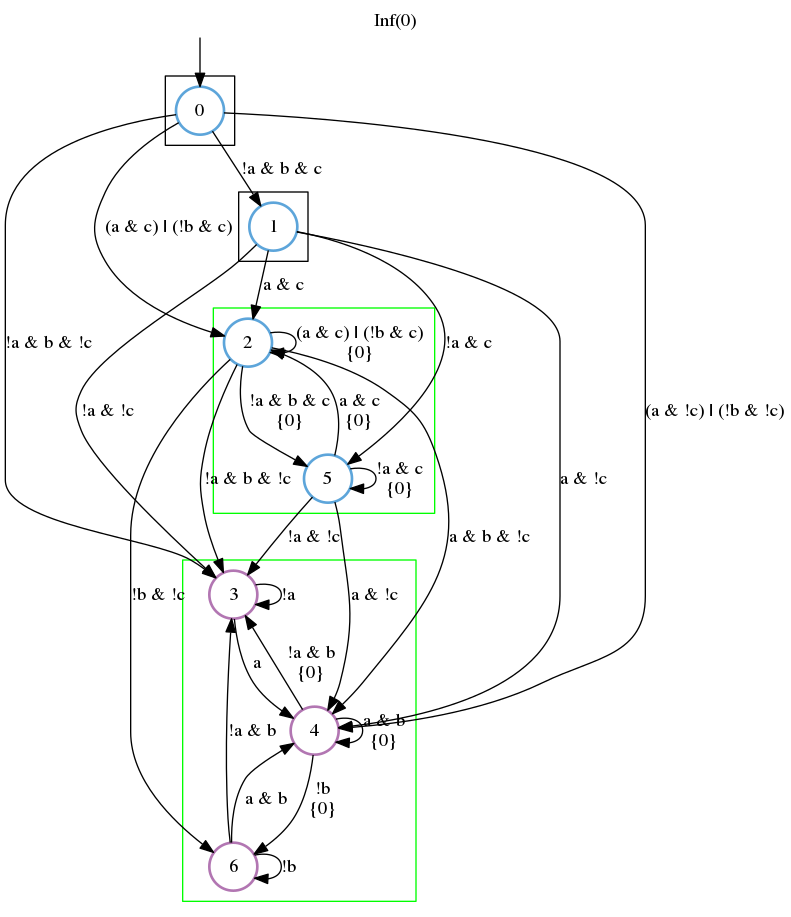
\includegraphics[scale=0.4]{img/highlight_language.png}
 \caption{An $\omega$-automaton colorized using \textbf{--hightlight-language} new option of
          \textbf{autfilt}}
 \label{fig:highlight_language}
\end{figure}

To come back to SAT-based minimization, by default, the binary search algorithm starts with 1 as
\textbf{min} value. Our theory is that the minimal automaton can not have less states than the total number
of languages recognized by each states. Instead of using 1 for \textbf{min} value, we set it to the total
number of recognized languages. This worked, it improved in general binary search algorithm but in somes
cases, which are far from negligible, the default binary search method was still better. This leads to a
new command line option: \textbf{sat-langmap}. This option is not set by default.